% begin module squeeze-theorem-ex11
\begin{frame}
\begin{example}[Example 10, p. 110]
Show that $\lim_{x\rightarrow 0} x^2 \sin \frac{1}{x} = 0$.
\uncover<2->{
\[
\text{\alert{WRONG:}} \qquad \lim_{x\rightarrow 0}x^2 \sin \frac{1}{x} = \lim_{x\rightarrow 0}x^2 \cdot \lim_{x\rightarrow 0}\sin \frac{1}{x}
\]
Doesn't work because $\lim_{x\rightarrow 0} \sin \frac{1}{x}$ doesn't exist.
}
\begin{columns}[c]
\column{.4\textwidth}
\uncover<6->{%
\ 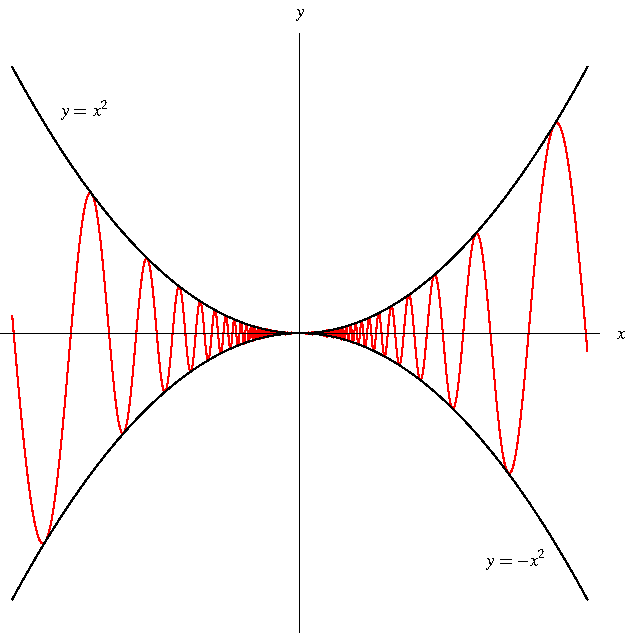
\includegraphics[height=4.5cm]{limits/pictures/02-03-ex11.pdf}%
}%
\column{.6\textwidth}
\uncover<3->{
\[
\begin{array}{rcccl}
-1 & \leq & \sin\frac{1}{x} & \leq & 1.\\
\uncover<4->{%
-x^2%
}&%
\uncover<4->{%
\leq %
}&%
\uncover<4->{%
x^2\sin\frac{1}{x}%
}&%
\uncover<4->{%
\leq %
}&%
\uncover<4->{%
x^2.%
}%
\end{array}
\]
}
\uncover<5->{
\[
\lim_{x\rightarrow 0} x^2 = 0 \qquad \text{and}\qquad  \lim_{x\rightarrow 0}(-x^2) = 0.
\]
}

\uncover<6->{
Therefore by the Squeeze Theorem
%Take $f(x) = -x^2, g(x) = x^2\sin\frac{1}{x}$, and $h(x) = x^2$. 
\belowdisplayskip=0pt
\abovedisplayskip=0pt
\[
\lim_{x\rightarrow 0}x^2\sin \frac{1}{x} = 0.
\]
}
\end{columns}

\end{example}
\end{frame}
% end module squeeze-theorem-ex11
